\documentclass[sigconf=true, nonacm=false, review=true, anonymous = false,screen=true]{acmart}
\usepackage{soul}

% This is not the correct ref format but it shows the refs in the text more clearly
% Have to be removed before submitting
%\setcitestyle{authoryear}
%\setcitestyle{citesep={;}}
\copyrightyear{2023}
\acmYear{2023}
% \setcopyright{acmlicensed}
\setcopyright{none}
\acmConference[GECCO '23]{2023
Genetic and Evolutionary Computation Conference}{July 10--14,
2023}{Lisbon, Portugal}
\acmBooktitle{2023 Genetic and Evolutionary Computation Conference
 (GECCO '23), July 10--14, 2023, Lisbon, Portugal}
\acmPrice{15.00}
%%
%% Submission ID.
%%\acmSubmissionID{123-A56-BU3}
\newcommand{\dv}[1]{\textbf{\textcolor{blue}{Diederick: #1}}}
\newcommand{\ak}[1]{\textcolor{violet}{\textbf{Anna:} #1}}
%%
%% end of the preamble, start of the body of the document source.
\begin{document}

%%
%% The "title" command has an optional parameter,
%% allowing the author to define a "short title" to be used in page headers.
\title[Performance of modular CMA-ES on strict box constrained problems]{Performance of modular CMA-ES on strict box constrained problems in the SBOX-COST benchmarking suite} %\\example submission for a short paper in the SBOX-COST workshop

%%
%% authors
\author{Diederick Vermetten}
\affiliation{%
    \institution{LIACS, Leiden University}
    \streetaddress{Niels Bohrweg 1}
    \city{Leiden}
    \postcode{2333}
    \country{The Netherlands}}
\email{d.l.vermetten@liacs.leidenuniv.nl}
\orcid{0000-0003-3040-7162}

\author{Olaf Mersmann}
\affiliation{%
  \institution{TH Köln}
  \city{Köln}
  \country{Germany}}
\email{olaf.mersmann@th-koeln.de}
\orcid{0000-0002-7720-4939}

\author{Manuel López-Ibáñez}
\affiliation{%
    \institution{University of Manchester}
    \city{Manchester}
    \country{UK}}
\email{manuel.lopez-ibanez@manchester.ac.uk}
\orcid{0000-0001-9974-1295}

\author{Youngmin Kim}
 \affiliation{%
    \institution{University of Manchester}
    \city{Manchester}
    \country{UK}}
\email{youngmin.kim@manchester.ac.uk}
\orcid{0000-0002-7699-6532}

\author{Richard Allmendinger}
 \affiliation{%
    \institution{University of Manchester}
    \city{Manchester}
    \country{UK}}
\email{richard.allmendinger@manchester.ac.uk}
\orcid{0000-0003-1236-3143}

\author{Anna V. Kononova}
\affiliation{%
      \institution{LIACS, Leiden University}
      \streetaddress{Niels Bohrweg 1}
      \city{Leiden}
      \postcode{2333}
      \country{The Netherlands}}
\email{a.kononova@liacs.leidenuniv.nl}
\orcid{0000-0002-4138-7024}

%%
%% By default, the full list of authors will be used in the page
%% headers. Often, this list is too long, and will overlap
%% other information printed in the page headers. This command allows
%% the author to define a more concise list
%% of authors' names for this purpose.
%\renewcommand{\shortauthors}{Trovato and Tobin, et al.}

%%
\begin{abstract}
This paper evaluates several versions of CMA-ES on the strict-box-constrained  benchmarking suite (SBOX-COST). SBOX-COST is a variant of the well-known BBOB benchmark suite that enforces box-constraints by returning an invalid evaluation value for solutions violating any of the constraints on the bounds of decision variables. We compare four variants of CMA-ES: two initialization methods (centre of mass near the origin versus uniformly at random) and two box-constraint handling methods (saturate versus no handling at all). Contrary to what may be expected, handling box-constraints by saturation is not always better that not handling them at all. However, over all BBOB functions, saturation is better than not handling and the difference increases with the number of dimensions. Enforcing sbox-constraints also has a clear negative effect on the performance of classical CMA-ES (with uniform random initialization and no constraint handling), especially as problem dimensionality increases.
\end{abstract}


%%
%% The code below is generated by the tool at http://dl.acm.org/ccs.cfm.
%% Please copy and paste the code instead of the example below.
%%
\begin{CCSXML}
<ccs2012>
   <concept>
       <concept_id>10003752.10010070.10011796</concept_id>
       <concept_desc>Theory of computation~Theory of randomized search heuristics</concept_desc>
       <concept_significance>500</concept_significance>
       </concept>
   <concept>
       <concept_id>10003752.10003809.10011254</concept_id>
       <concept_desc>Theory of computation~Algorithm design techniques</concept_desc>
       <concept_significance>500</concept_significance>
       </concept>
 </ccs2012>
\end{CCSXML}

\ccsdesc[500]{Theory of computation~Theory of randomized search heuristics}
\ccsdesc[500]{Theory of computation~Algorithm design techniques}

\ccsdesc[300]{Mathematics of computing~Evolutionary algorithms}
\ccsdesc[500]{Theory of computation~Discrete optimization}

%%
%% Keywords.
\keywords{keyword, keyword}

%%
%% This command processes the author and affiliation and title
%% information and builds the first part of the formatted document.
\maketitle

\section{Introduction}
Box-constraints impose limits on the domain of decision variables and are perhaps the most typical type of constraints that arise in black-box continuous optimization. In almost all real-world problems, the range of decision variables will be limited by physical, design, resource or policy bounds that are known a priori. As a result of these bounds, solutions outside those bounds, i.e., violating the box-constraints, are not only unacceptable, but they may not have a defined value of the objective function. Unfortunately, many optimization algorithms do not follow this assumption and, instead, allow the evaluation of solutions violating box-constraints. Moreover, benchmarking suites used for comparing algorithms, such as COCO/BBOB~\cite{hansen2020coco}, return a valid objective value for such solutions, which is used by the algorithms to steer their search.

Here, we consider a benchmark SBOX-COST that enforces box-constraints by returning the same invalid value ($\infty$) for any infeasible solution, thus the algorithm cannot use infeasible solutions to inform the search. We evaluate the effect that such strict-box-constraints have on the performance of some variants the Covariance Matrix Adaptation Evolution Strategy (CMA-ES).

The Covariance Matrix Adaptation Evolution Strategy (CMA-ES)~\cite{Hansen.1996} is a very popular heuristic optimisation algorithm for continuous optimisation problems~\cite{vermetten_gecco2022}. CMA-ES is considered state-of-the-art in evolutionary computation and has been adopted as one of the standard tools for continuous optimisation in many research labs. There are many flavours and variants of CMA-ES developed through the years and different implementations of sub-components such as the sampling strategy and the boundary correction method.

In recent works, the different modules and configurations of CMA-ES are explored and analysed based on their performance~\cite{de2021tuning}. In that research a modular CMA-ES framework is presented, representing a plethora of different CMA-ES configurations. In this paper, the modular CMA-ES framework is used to analyse the effect of introducing boundaries to standard BBOB problems, as done in the new SBOX-COST benchmark. 

This paper serves as an \textit{example} of a short paper for the ACM Workshop on Strict Box-Constrained Optimization\footnote{\url{https://sbox-cost.github.io/}} (SBOX-COST) within GECCO~2023.

\section{Methodology}
\subsection{SBOX-COST benchmarking suite}

For our benchmarking, we make use of the newly proposed Strict Box-Constraint Optimization Studies benchmark\footnote{\url{https://github.com/sbox-cost}} (SBOX-COST), which is a modification of the original BBOB suite~\cite{hansen2020coco}. The changes made are as follows: 
\begin{itemize}
    \item \textit{hard box-constraints}: points evaluated outside of the domain $[-5,5]^d$ are considered infeasible and evaluated to $\infty$;
    \item Location of the optima: SBOX-COST has optima across instances located uniformly within the full domain -- except for, as in BBOB, F4, F8, F9, F19, F20, F24 which have optima uniform in $[-4,4]^d$ and F5 - in some corners of $[-5,5]^d$.
\end{itemize} 

\subsection{Modular CMA-ES}
To investigate several commonly and less commonly used configurations and variants of the CMA-ES algorithm~\cite{Hansen.1996}, we use the Modular CMA-ES framework~\cite{van2017algorithm,de2021tuning}. The framework is open-source and available\footnote{\url{https://github.com/IOHprofiler/ModularCMAES}} as part of the IOHprofiler \cite{doerr2018iohprofiler} environment. 

Modular CMA-ES framework is currently made up of $11$ modules, each having a number of implemented options: Active update (2), Elitism (2), Orthogonal Sampling (2), Sequential Selection (2), Threshold Convergence (2), Step-Size adaptation (7), Mirrored Sampling (3), Quasi-Gaussian Sampling (3), Recombination Weights (2), Restart Strategy (3) and Boundary Correction (6). The framework allows a total of $72.576$ possible configurations. A detailed description of each module and their settings can be found in~\cite{de2021tuning}.

In this paper, to investigate the \textit{effect of the introduction of strict boundaries} on the BBOB problems in the SBOX-COST benchmarking suite, we compare the behaviour of 4 different variants withing modular CMA-ES by considering:
\begin{itemize}
    \item two \textit{initialization} methods for the centre of mass (set to the origin of the space, \texttt{centre}, or set uniformly at \texttt{random} in the domain),
    \item enabling or disabling the method for dealing with \textit{box-constraints} (\texttt{saturate}, which places the infeasible coordinates to the closest corresponding bound or \texttt{none} which allows infeasible points ). 
\end{itemize} 
All \textit{other modules} and parameter settings are set to their defaults specified in~\cite{de2021tuning}. 

\begin{figure}[!tb]
 \centering
 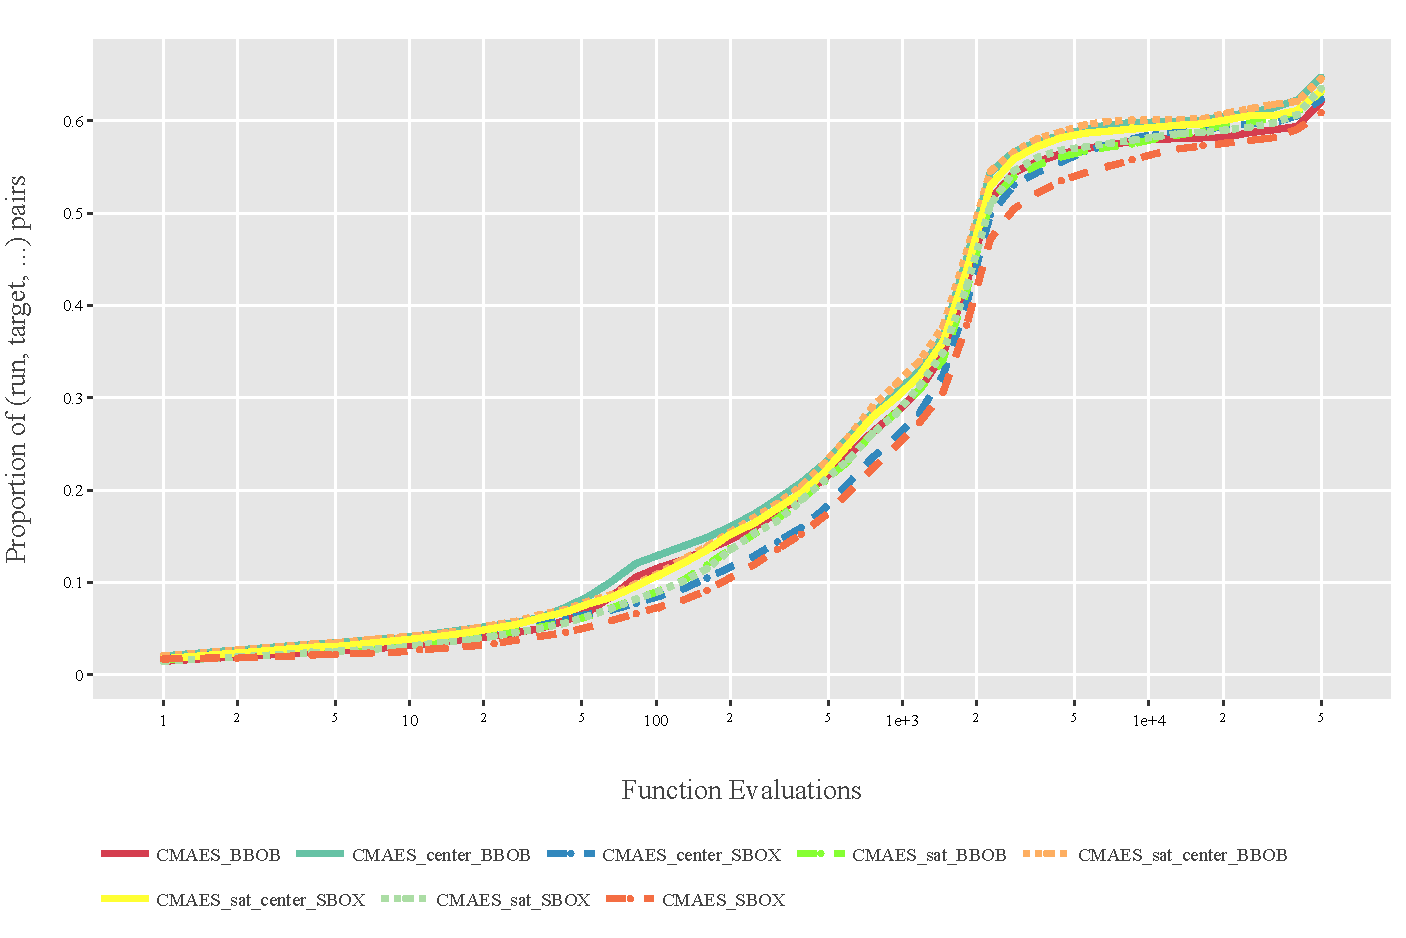
\includegraphics[width=.95\linewidth,trim=1mm 5mm 13mm 9mm,clip]{Figures/ECDF_5D_CMAESS.pdf}
 \caption{Empirical Cumulative Distribution Function for all considered variants within modular CMA-ES, aggregated over the 24 functions of BBOB and SBOX-COST in 5D. Targets are 51 log-spaces values between $10^2$ and $10^{-8}$ ('bbob' default in IOHanalyzer).}\label{fig:res_ecdf}
\end{figure}
\section{Experimental setup}
We evaluate algorithms on the same 24 functions of both BBOB and SBOX-COST. The only difference between a function in both benchmark suites is the objective function value returned for solutions violating a box constraint.
We use an identical setup for BBOB and SBOX-COST: 15 instances per function, 1 run per instance, dimensionality $d\in\{5, 20, 40\}$, budget $10000\times d$.

Experiments reported in this study are carried out in the IOHex\-pe\-ri\-men\-ter environment~\cite{de2021iohexperimenter}, which implements both sets of benchmarking functions. 

\section{Results}
\begin{figure}[!tb]
 \centering
 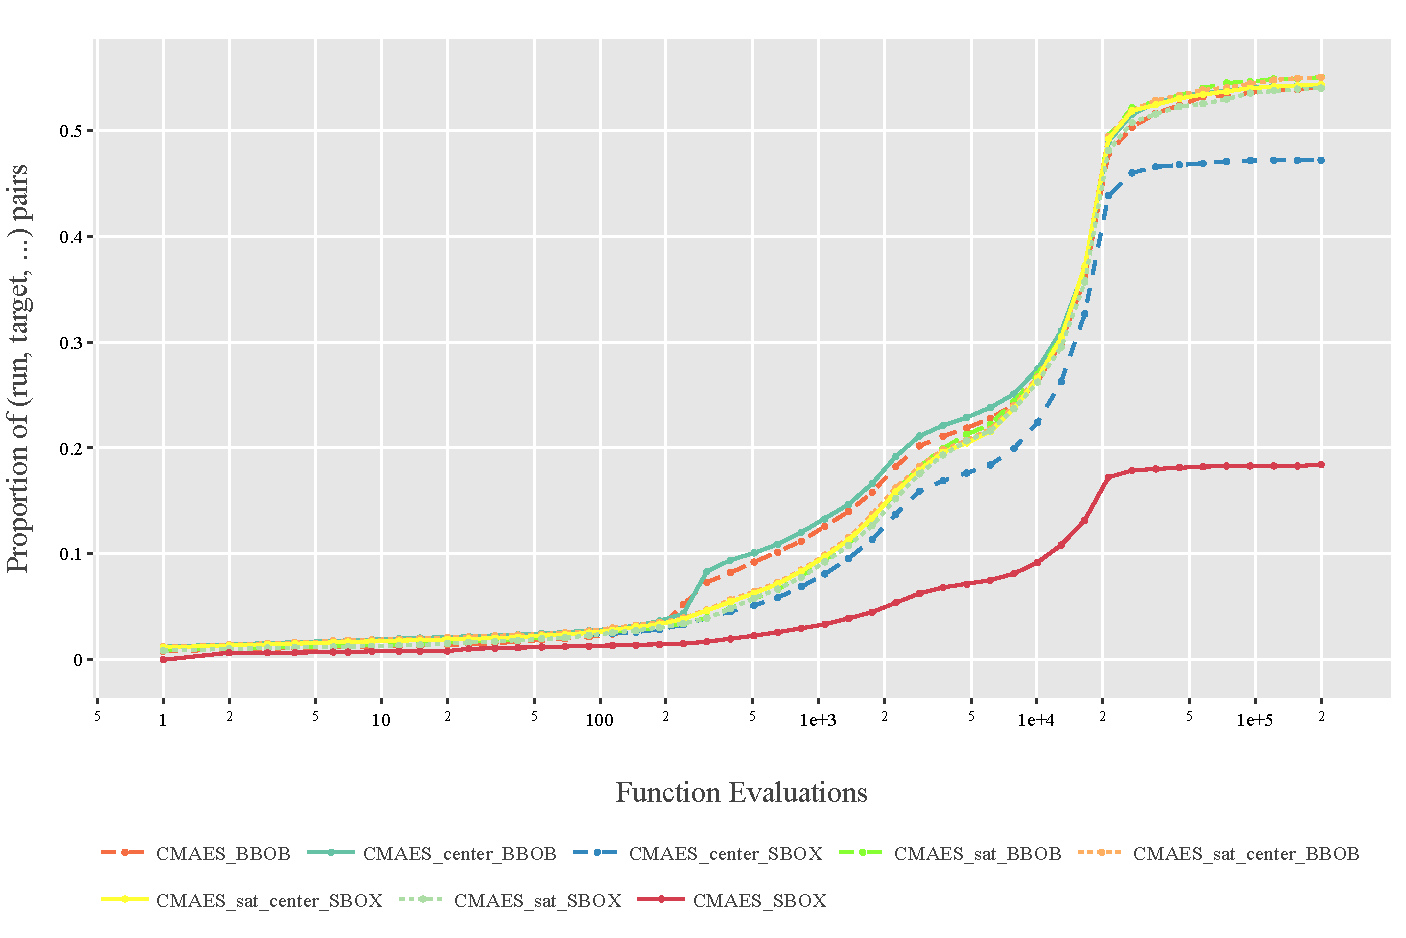
\includegraphics[width=.95\linewidth,trim=1mm 5mm 13mm 9mm,clip]{Figures/ECDF_20D_CMAESS.pdf}
 \caption{Empirical Cumulative Distribution Function for all considered variants within modular CMA-ES, aggregated over the 24 functions of BBOB and SBOX-COST in 20D. Targets are 51 log-spaces values between $10^2$ and $10^{-8}$ ('bbob' default in IOHanalyzer).}\label{fig:res_ecdf2}
\end{figure}

\begin{figure*}
 \centering
 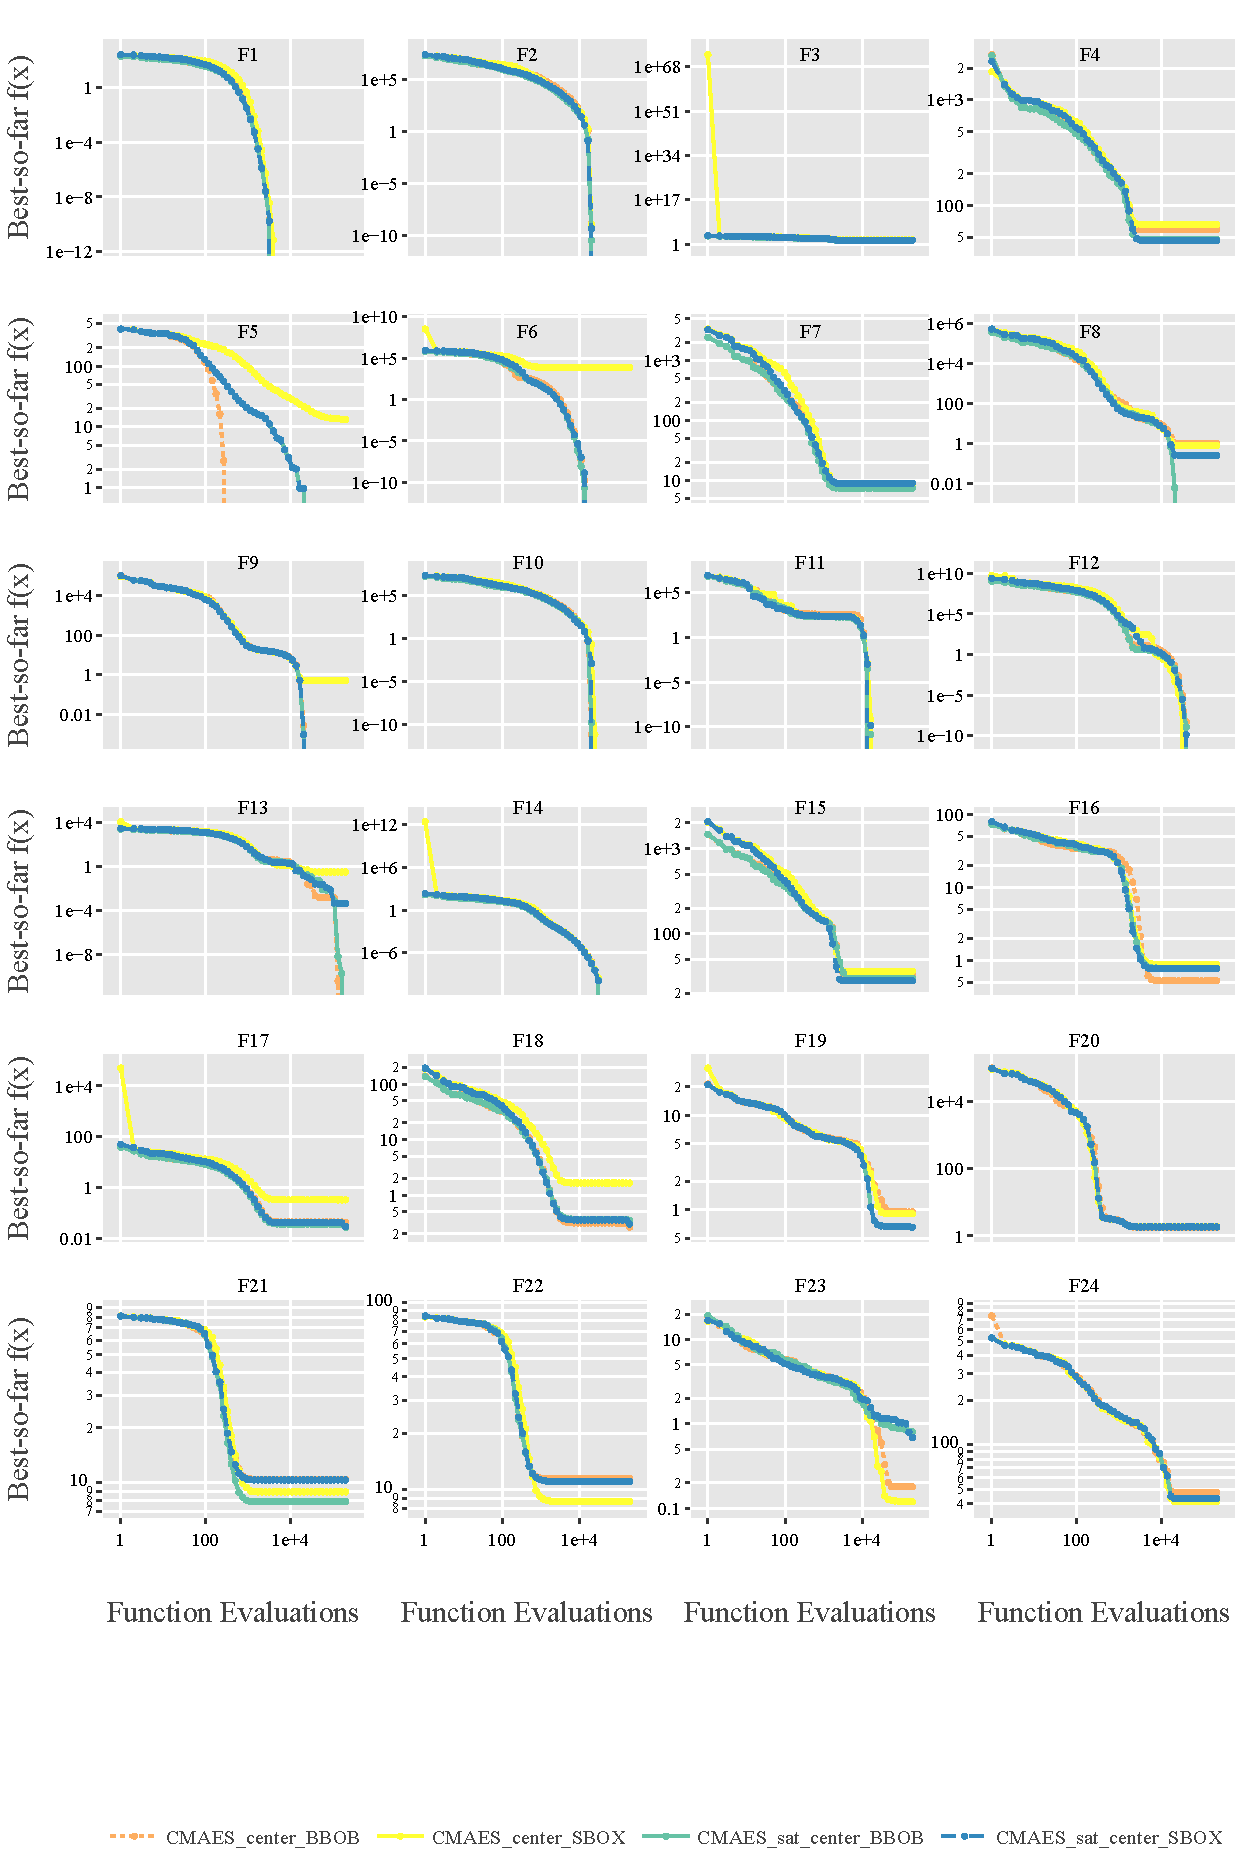
\includegraphics[width=.95\linewidth,trim=8mm 55mm 4mm 6mm,clip]{Figures/FCE_Mult-2023-03-30 (1).pdf}
 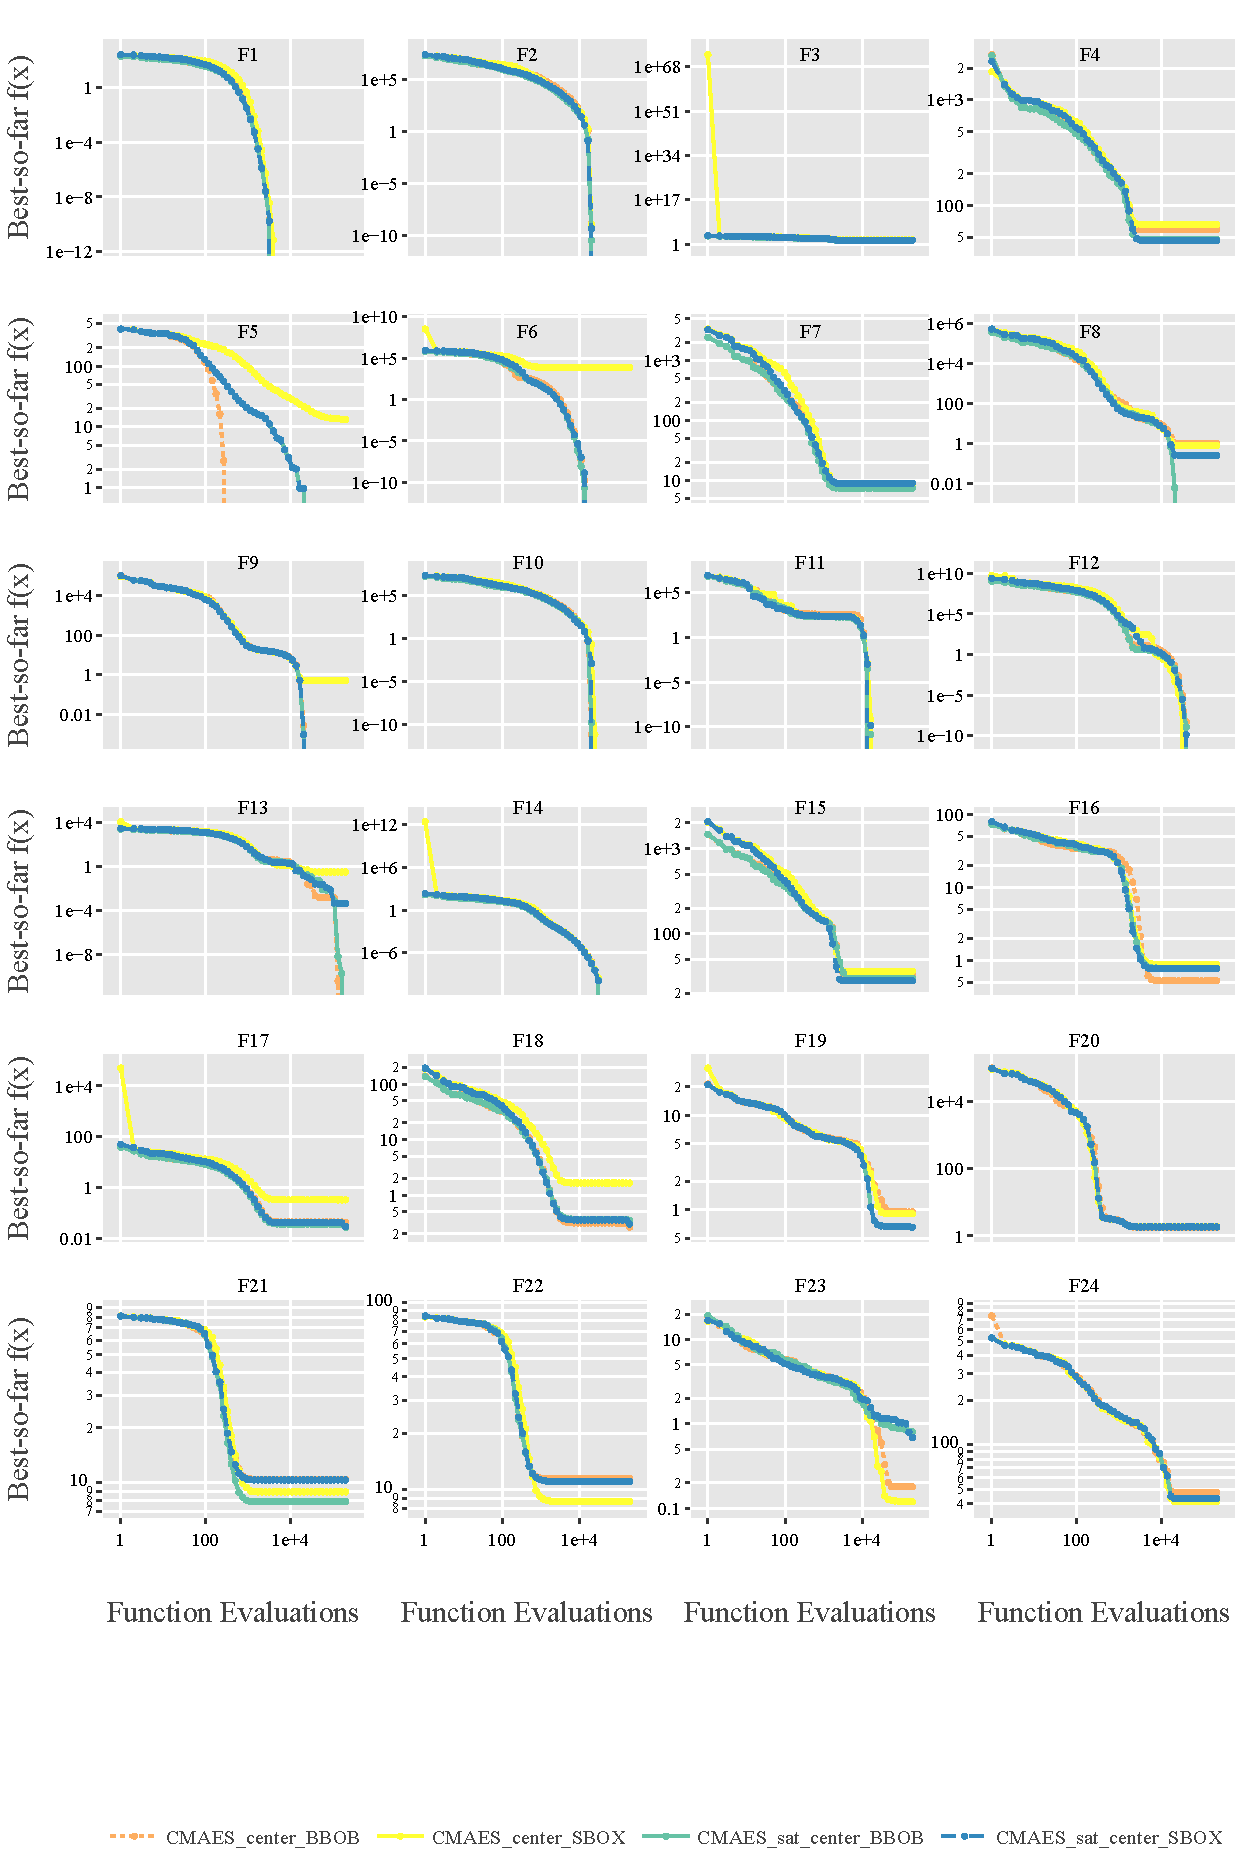
\includegraphics[width=.95\linewidth,trim=8mm 5mm 4mm 305mm,clip]{Figures/FCE_Mult-2023-03-30 (1).pdf}
 \caption{Mean function value over time for the CMA-ES methods with \texttt{centre} initialization, for 24 SBOX-COST functions of BBOB and SBOX-COST in 20D.}\label{fig:res_ert}
\end{figure*}

% latex table generated in R 4.1.2 by xtable 1.8-4 package
% Thu Mar 30 13:05:22 2023
\begin{table*}[!t]
\centering
\tiny
\begin{tabular}{rrrlrrrrrrrrrrrrrr}
  \hline
 & DIM & funcId & ID & runtime & runs & mean & median & sd & 2\% & 5\% & 10\% & 25\% & 50\% & 75\% & 90\% & 95\% & 98\% \\ 
  \hline
1 & 20 & 5 & CMAES\_center\_BBOB & 10000 &  15 & 0 & 0 & 0 & 0 & 0 & 0 & 0 & 0 & 0 & 0 & 0 & 0 \\ 
  2 & 20 & 5 & CMAES\_center\_SBOX & 10000 &  15 & 29.58 & 32.94 & 9.15 & 11.55 & 11.56 & 14.44 & 26.25 & 32.94 & 34.90 & 37.68 & 38.80 & 39.99 \\ 
  3 & 20 & 6 & CMAES\_center\_BBOB & 10000 &  15 & 0 & 0 & 0 & 0 & 0 & 0 & 0 & 0 & 0 & 0 & 0 & 0 \\ 
  4 & 20 & 6 & CMAES\_center\_SBOX & 10000 &  15 & 7735.90 & 0 & 29961.02 & 0 & 0 & 0 & 0 & 0 & 0 & 0 & 34811.56 & 83547.75 \\ 
  5 & 20 & 7 & CMAES\_center\_BBOB & 10000 &  15 & 7.56 & 7.42 & 3.59 & 1.58 & 2.11 & 3.43 & 5.73 & 7.42 & 8.93 & 11.74 & 13.80 & 14.59 \\ 
  6 & 20 & 7 & CMAES\_center\_SBOX & 10000 &  15 & 7.66 & 8.65 & 4.07 & 2.26 & 2.53 & 2.92 & 4.45 & 8.65 & 10.19 & 12.02 & 13.64 & 15.07 \\ 
  7 & 20 & 14 & CMAES\_center\_BBOB & 10000 &  15 & 0 & 0 & 0 & 0 & 0 & 0 & 0 & 0 & 0 & 0 & 0 & 0 \\ 
  8 & 20 & 14 & CMAES\_center\_SBOX & 10000 &  15 & 0 & 0 & 0 & 0 & 0 & 0 & 0 & 0 & 0 & 0 & 0 & 0 \\ 
  9 & 20 & 15 & CMAES\_center\_BBOB & 10000 &  15 & 33.70 & 32.83 & 11.75 & 14.61 & 17.11 & 20.10 & 25.87 & 32.83 & 42.78 & 47.16 & 50.54 & 53.05 \\ 
  10 & 20 & 15 & CMAES\_center\_SBOX & 10000 &  15 & 36.17 & 33.83 & 11.41 & 22.17 & 22.59 & 24.48 & 27.36 & 33.83 & 43.28 & 53.47 & 54.49 & 55.22 \\ 
  11 & 20 & 16 & CMAES\_center\_BBOB & 10000 &  15 & 0.52 & 0.39 & 0.44 & 0.10 & 0.11 & 0.12 & 0.17 & 0.39 & 0.73 & 1.10 & 1.38 & 1.51 \\ 
  12 & 20 & 16 & CMAES\_center\_SBOX & 10000 &  15 & 0.89 & 0.84 & 0.60 & 0.09 & 0.10 & 0.16 & 0.32 & 0.84 & 1.39 & 1.57 & 1.73 & 1.87 \\ 
  13 & 20 & 17 & CMAES\_center\_BBOB & 10000 &  15 & 0.04 & 0.03 & 0.04 & 0 & 0 & 0 & 0.02 & 0.03 & 0.06 & 0.09 & 0.12 & 0.15 \\ 
  14 & 20 & 17 & CMAES\_center\_SBOX & 10000 &  15 & 0.33 & 0.08 & 0.67 & 0 & 0 & 0.01 & 0.02 & 0.08 & 0.25 & 0.76 & 1.46 & 2.12 \\ 
  15 & 20 & 18 & CMAES\_center\_BBOB & 10000 &  15 & 0.31 & 0.25 & 0.23 & 0.07 & 0.07 & 0.09 & 0.17 & 0.25 & 0.36 & 0.70 & 0.73 & 0.75 \\ 
  16 & 20 & 18 & CMAES\_center\_SBOX & 10000 &  15 & 1.65 & 1.58 & 1.18 & 0.33 & 0.34 & 0.43 & 0.73 & 1.58 & 2.34 & 2.84 & 3.38 & 4.11 \\ 
  17 & 20 & 21 & CMAES\_center\_BBOB & 10000 &  15 & 10.45 & 7.59 & 8.87 & 0 & 0 & 0.63 & 5.15 & 7.59 & 16.40 & 21.19 & 25.97 & 28.86 \\ 
  18 & 20 & 21 & CMAES\_center\_SBOX & 10000 &  15 & 8.92 & 7.59 & 6.71 & 1.06 & 1.61 & 2.02 & 3.21 & 7.59 & 12.34 & 17.11 & 19.15 & 22.01 \\ 
  19 & 20 & 22 & CMAES\_center\_BBOB & 10000 &  15 & 11.50 & 7.27 & 14.07 & 1.05 & 1.58 & 1.95 & 3.51 & 7.27 & 14.58 & 20.38 & 32.28 & 46.99 \\ 
  20 & 20 & 22 & CMAES\_center\_SBOX & 10000 &  15 & 8.65 & 5.06 & 7.93 & 1.05 & 1.58 & 1.95 & 2.59 & 5.06 & 12.86 & 20.38 & 22.89 & 24.44 \\ 
  21 & 20 & 23 & CMAES\_center\_BBOB & 10000 &  15 & 2.24 & 2.62 & 1.14 & 0.15 & 0.19 & 0.38 & 1.71 & 2.62 & 3.05 & 3.36 & 3.39 & 3.41 \\ 
  22 & 20 & 23 & CMAES\_center\_SBOX & 10000 &  15 & 1.82 & 2.49 & 1.41 & 0.07 & 0.07 & 0.09 & 0.12 & 2.49 & 2.99 & 3.22 & 3.32 & 3.44 \\ 
   \hline
\end{tabular}
\caption{Summary statistics of function value reached after $10\,000$ evaluations for the CMA-ES with center initialization and no boundary correction on a selected set of 20-dimensional problems.}\label{tab:fce}
\end{table*}



The data from the described experiments is visualized using IOHanalyzer~\cite{IOHanalyzer}. We start by aggregating the performance of each of the 8 settings across all 5-dimensional problems. This is done by making use of the Empirical Cumulative Distribution function, which aggregates the fraction of targets (we use the default of 51 logarithmically spaced targets $\{10^{-8}\dots10^{2}\}$) hit in each run on each function, as shown in Figure~\ref{fig:res_ecdf}. From this figure, we notice that the variants of CMA-ES without boundary correction run on the SBOX-suite perform slightly worse on aggregate than the other versions. 

In Figure~\ref{fig:res_ecdf2}, we show the ECDF curves on the 20-dimensional problems. Here, the poor performance of the CMA-ES with random initialization without boundary correction on SBOX is much more obvious. This is likely caused by the fact that in higher dimensions, a Gaussian distribution around a random point will be much more likely to generate points outside the domain, leading to many wasted function evaluations, and potentially a disrupted search process. While initializing the CMA-ES in the center of the domain alleviates this problem somewhat, it still performs worse than the versions which add a boundary handling mechanism. 

To get a more detailed view of the performance on individual functions, we plot the convergence trajectories (mean function value over time) in Figure~\ref{fig:res_ert}. To ease readability, we only show the CMA-ES variants which are initialized in the center of the domain. From this figure, we can see that for several functions, the performance differences between the algorithms run on SBOX and on BBOB are rather small. In particular, this is the case for the functions $\{4, 8, 9, 19, 20, 24\}$, where the instance generation procedure was not modified from the original BBOB suite. However, the differences on function $5$ clearly show the impact of the hard box-constraint, with the CMA-ES on BBOB easily solving the problem (achieved by moving outside the domain).

Finally, for a few selected functions, we show some detailed summary statistics in Table~\ref{tab:fce}, which confirms the observations from Figure~\ref{fig:res_ert}: for many problems, the CMA-ES can overcome the addition of hard box-constraints and changed function initialization, although there are some problems where the changes lead to a noticeable deterioration in performance.\footnote{Note that the discussion in this paper is purely for illustration purposes. In a submitted paper, this should be extended. }


\section{Conclusions}

In this paper we have benchmarked four variants of CMA-ES on SBOX-COST, which is a variant of the BBOB suite that enforces box-constraints. Our results clearly show that enforcing box-constraints has a negative effect on the performance of classical CMA-ES, specially with higher dimensionality. Although not handling box-constraints sometimes performs worse than the constraint handling method evaluated here (saturation), over all BBOB functions, handling box-constraints is clearly better than ignoring them when the box-constraints are strict.


\section*{Reproducibility}
To ensure the reproducibility of results presented in this paper, the complete code used for experiments and runs data in the IOH format have been uploaded to a Zenodo repository.\footnote{\url{https://doi.org/10.5281/zenodo.7649077}}

%%
%% The acknowledgments section is defined using the "acks" environment
%\begin{acks}
%\hl{anything?}
%\end{acks}

%%
%% The next two lines define the bibliography style to be used, and
%% the bibliography file.
\bibliographystyle{ACM-Reference-Format}
\bibliography{references}

\end{document}

%%% Local Variables:
%%% mode: latex
%%% TeX-master: t
%%% End:
